\chapter{Introdution}

With this new part, we will get to discover a new way to approach business processes and help
improve our business, it has its own unique way that is different from ERP approach but to get BPM
approach we will need to understand what a business process is.\\\\
A business process is an activity or set of activities that can accomplish a specific organizational goal.
Business processes should have purposeful goals, be as specific as possible, and have consistent
outcomes. It is a collection of activities that takes one or more kinds of input and creates an output,
such as a report or forecast, that is of value to the customer.\\\\
ERP software supports executing business processes by supporting the efficient operation of business
processes by integrating tasks related to sales, marketing, manufacturing, logistics, accounting, and
staffing—throughout a business. In addition to this cross-functional integration, which is at the heart
of an ERP system, companies connect their ERP systems, using various methods, to coordinate
business processes with their customers and suppliers.\\\\
So how does BPM come in the picture? Business Process Management (BPM) is an approach that
focuses on capturing and improving business processes to make an organization more efficient. This
can be achieved by first capturing an organizations’ current-state end-to-end processes and then
documenting the steps in process maps.\\\\
While the ERP job cares more about cross-functional integration and tends to be limited to
organizational functions, BPM job tends to be much more process-focused.\\\\
Most companies, when undertaking a business improvement initiative, will consider implementing a
dedicated BPM system to help them model, analyze, and optimize processes to drive the business
transformation forward.\\\\
BPM tends to be flexible with approaching business processes design. It can manipulate, change, fix
and monitor a business process easily. The usual cycle of BPM fig \ref{fig:bpm_flow} helps to achieve this
flexibility which includes
\begin{figure}[h]
    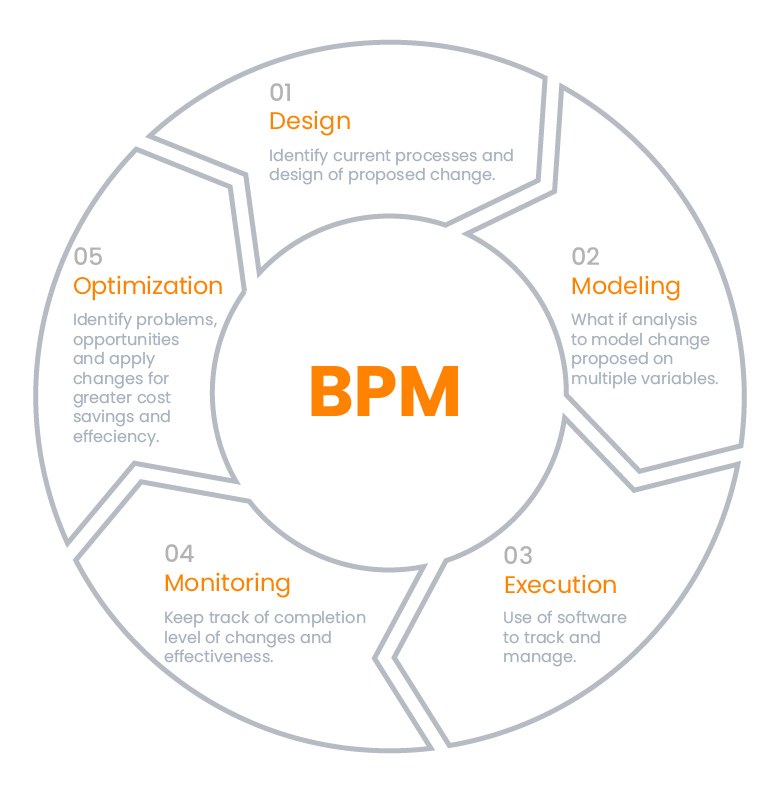
\includegraphics[width=80mm]{bpm_flow}
    \centering
    \caption{BPM Cycle}
    \label{fig:bpm_flow}
\end{figure}
\begin{itemize}
    \item \textbf{Design} Process design encompasses both the identification of existing processes and the
    design of future processes. Areas of focus include representation of the process flow, the
    factors within it, alerts and notifications, escalations, standard operating procedures, service
    level agreements, and task hand-over mechanisms
    \item \textbf{Modeling} Modeling takes theoretical design and introduces combinations of variables. For
    example, changes in rent or materials costs, which determine how the process might operate
    under different circumstances.
    \item \textbf{Monitoring} Monitoring encompasses the tracking of individual processes, so that
    information on their side can be easily seen, and the status of their performance of one or
    more processes can be provided. In addition, this information can be used to work with
    customers and suppliers to improve their connected processes and measures information of
    three categories: cycle time, defect rate, and productivity
    \item \textbf{Optimization} Process optimization includes retrieving process performance information
    from modeling or monitoring phase; identifying the potential or actual bottlenecks and the
    potential opportunities for cost savings or other improvements; and then, applying those
    enhancements in the design of the process. Process mining tools are able to discover critical
    activities and bottlenecks, creating greater business value
    
\end{itemize}



We mentioned that BPM helps capture end-to-end processes, but \textbf{what does end-to-end process really
mean}\\\\
What end-to-end process really means is from start to finish. The goal is to understand and thus to assess and improve an entire process —not just its components.
\\\\

\section{What is a process ?}
A process is a sequence of tasks. Every task is an action, and is carried out by a person
or by some automatic system. All processes share certain characteristics\\

\textbf{\textit{Interaction over time}}
\begin{adjustwidth}{2cm}{}
    A chronological relationship between tasks, with due dates and sequencing but
not a schedule.\\\\\\
\end{adjustwidth}
\textbf{\textit{Multiple actors}}
\begin{adjustwidth}{2cm}{}
    More than one person or automatic system must complete tasks for the whole
process to be successful.\\
\end{adjustwidth}
\textbf{\textit{Repetition}}
\begin{adjustwidth}{2cm}{}
    The sequence of tasks is repeated, either at fixed intervals or when triggered by a
specific event.
\end{adjustwidth}

\section{What Is Not a Process ?}
The action of filling out a form is not a process. A form that has many pages and is
filled out online is a single task for a single user. A form that can be filled out in more
than one sitting is a single task for a single user. Even a form that has smart fields that
depend on other fields, with conditional display, is a single task for a single user.
A state diagram is not a process. A process is constructed from actions. The things
that are updated by these actions might have states associated with them, so you
might create state diagrams as part of your process validation, but the state diagram is
not itself a process.

\chapter{The BPM}

Yet again we have a name for our implementation of BPM that we will use over the next few chapters
and it follows the same pattern for our naming schemes, \textbf{“The BPM”}.\\\\
The BPM is meant to work best when integrated with other applications to be used to its potential. It
will provide all the tools to be used inside other programs. But it still works as a full Standalone BPM
solution to design, execute and monitor Business processes.\\\\
It offers a pipeline that works on three stages each can work as a standalone application, the pipeline
works as follows
\begin{itemize}
    \item Design business process using a graphical application
    \item Execute the business process with the ability to modify its execution at runtime
    \item Monitor the business process and see the process execution in detail and change the execution
    graphically
\end{itemize}

\section{The Process}

For each process The starting conditions and timetable of a process. The following question need to be considered\\\\
Under what conditions will the process start ? These conditions were referenced from the book Process-Driven Applications \cite{processbpmn}\\
\begin{itemize}
    \item \textbf{Time}\\
    The process starts at a particular time\\
    The process starts after a particular time interval\\
    The process starts in relation to another time\\
    \item \textbf{Conditions}\\
    The process starts once one or more conditions are met, for example, a
    warehouse is restocked with a particular product once stock levels go
    below a predefined threshold value.
    \item \textbf{Messages}\\
    The process waits for a particular message to arrive.
    \item \textbf{Events}\\
    Events have an important role, especially in exception situations. An event
is triggered when an extraordinary situation arises that requires special handling, for example, a late delivery, a machine failure, an accident, or Similar.
\end{itemize}

After the designer answers these questions, he will change the setting of the starting node to satisfy
the conditions required for this process.\\\\
For each process, there will be three start nodes, two of which will have their starting conditions
embedded in them
\begin{itemize}
    \item The first will be triggered when the process loaded in the engine can be used to
    initialize data related to the process or when integrated with a GUI application that
    can be used to generate a GUI for the process when loaded.
    \item The second will be when the process awakes and starts to run, whether it is its first
    time to run or awaken after a pause, can be used to get data to memory back before
    continuing the process.
    \item The third will be the one which will start based on the question that the user answered
    and can choose which event will make it start.
   \end{itemize}

\subsection{Involved Process Roles}
The involved process roles define who is responsible for performing which
activities during the process. All you need is a simple list of process roles and a
description of the functions the roles perform within the process. At runtime, users
and groups from the company’s user management solution are assigned to these
roles. Although this presents a challenge, the complex task of assigning users to
process roles in workflow management systems within company organizations is
outside the scope of this book and is not discussed in more detail here.

\section{Notation}
While designing our notation we came across two other notations that are used as standards like\\\\

\textbf{BPMN 2.0} \cite{OMG-BPMN} (Business Process Model and Notation), it provides
businesses with the capability of understanding their internal business procedures in a graphical
notation and will give organizations the ability to communicate these procedures in a standard
manner.\\\\
\textbf{BPEL} \cite{OASIS-BPEL} (Business Process Execution Language) is an XML based language that allows Web services
in a service-oriented architecture (SOA) to interconnect and share data.\\\\
Our notation is affected deeply by BPMN 2.0, but our goal was simplicity so we removed some of its
complexity and added some other nodes that can be used in an easy and intuitive manner, So while
BPMN 2.0 is much capable of executing complex business processes. Our notation is much more
simpler to use and understand.

\subsection{The Nodes}
They should be descriptive enough to understand business process like interaction with users and
repetition of tasks, simple to be intuitive to use and have the ability to be extended for advanced
usage. \\\\

\large \textbf{Start}\\

\begin{tabular}{C{2.2cm}  L{15cm}}
    
\includegraphics[width=\linewidth]{start} & Specifies the start of the flow.\newline Each flow will have three start nodes,
    OnLoaded - OnAwake - OnStart. \newline
    The latter must be explicitly defined.\newline
The others will be implicitly defined to do nothing if not explicitly
defined.
\end{tabular}

\break

\large \textbf{End}\\

\begin{tabular}{C{2.2cm}  L{15cm}}
    
\includegraphics[width=\linewidth]{end} & Specifies the end of a flow or just a branch from the flow.
    \newline Each flow can have one or more than one end node.
    \newline Each will be the end of one flow or more than one.
    \newline You can specify logging for each end to specify what ended.
defined.
\end{tabular}

\par\vspace {1cm}

\large \textbf{Service Task}\\

\begin{tabular}{C{2.2cm}  L{15cm}}
    
\includegraphics[width=\linewidth]{task} & Executes Web services based on REST.
    \linebreak Will Create the request and handle the response.
defined.
\end{tabular}

\par\vspace {1cm}

\large \textbf{Database}\\

\begin{tabular}{C{2.2cm}  L{15cm}}
    
\includegraphics[width=\linewidth]{database} & Works with an SQL database to connect, modify and get data.
    \linebreak Can work with different SQL implementation (Oracle - MySQL - SQLite).
    \linebreak Can listen to the database for data insertion using polling.
    \linebreak Provides the user with a way to visualize the database while choosing a
    query to execute, like showing the table and data.
defined.
\end{tabular}

\par\vspace {1cm}

\large \textbf{Parallel}\\

\begin{tabular}{C{2.2cm}  L{15cm}}
    
\includegraphics[width=\linewidth]{parallel} & Makes more than one flow to be executed in the same process.
    \linebreak The two flows will be executed at the same time in the same environment
    using parallel processing.
defined.
\end{tabular}

\par\vspace {1cm}

\large \textbf{Condition}\\

\begin{tabular}{C{2.2cm}  L{15cm}}
    
\includegraphics[width=\linewidth]{condition} & Divides the flow into more than one flow, each with a condition.
    \linebreak When the flow reaches this node, it will evaluate the condition to which
    flow and will choose the flow that evaluates the condition to true.
defined.
\end{tabular}

\par\vspace {1cm}

\large \textbf{External Event}\\

\begin{tabular}{C{2.2cm}  L{15cm}}
    
\includegraphics[width=\linewidth]{task} &Executes Events from outside of The BPM nodes.
defined.
\end{tabular}

\par\vspace {1cm}

\large \textbf{Timer Event}\\

\begin{tabular}{C{2.2cm}  L{15cm}}
    
\includegraphics[width=\linewidth]{timer} &Waits for a certain time before proceeding with the flow.
\end{tabular}

\par\vspace {1cm}

\large \textbf{Script}\\

\begin{tabular}{C{2.2cm}  L{15cm}}
    
\includegraphics[width=\linewidth]{script} &Executes a predefined script written by user to add functionality to The
    BPM.
\end{tabular}

\par\vspace {1cm}

\large \textbf{Json}\\

\begin{tabular}{C{2.2cm}  L{15cm}}
    
\includegraphics[width=\linewidth]{json} &Creates a JSON string or get the values of the elements in a java string.
\end{tabular}

\par\vspace {1cm}

\large \textbf{Increment Function}\\

\begin{tabular}{C{2.2cm}  L{15cm}}
    
\includegraphics[width=\linewidth]{add} &A function that increase variable by 1 used in loops
\end{tabular}


\section{Tasks}

Tasks are the main components of The BPM. Each business process will have a variety of tasks that
need to be executed. The BPM supports different kinds of tasks.

\begin{itemize}
    \item \textbf{API Tasks} \\
    They are tasks that are defined through an API which is a defined interface of how to interact
    with other applications functions. It can be used to add functionality to The BPM by
    executing functions available at other places
    \item \textbf{Script Tasks} \\
    They are tasks that are defined through an API which is a defined interface of how to interact
    with other applications functions. It can be used to add functionality to The BPM by
    executing functions available at other places
    \item \textbf{User Tasks} \\
    A User Task is used to model work that needs to be done by a human actor like filling a form
or accepting a request.

\begin{figure}[h]
    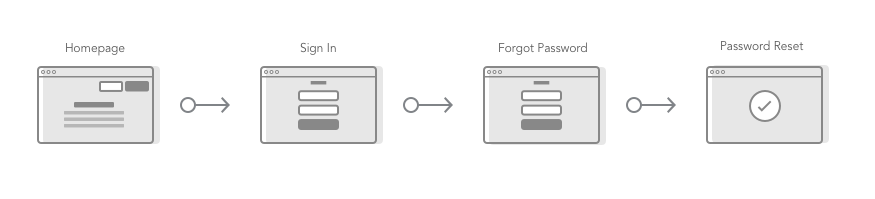
\includegraphics[width=\linewidth]{user_task}
    \centering
    \caption{User Task}
    \label{fig:user_task}
\end{figure}

    \item \textbf{External Tasks} \\
    They are tasks that are only known to the business, and they have no defined way of accessing
them from outside of the system, so the only way to execute them is by executing them inside
of the system, So The BPM will define a way to define the tasks by the names known to the
business and will put them in a Queue waiting for the system to look for them and get them
then execute them. Fig \ref{fig:task_worker}

\begin{figure}[h]
    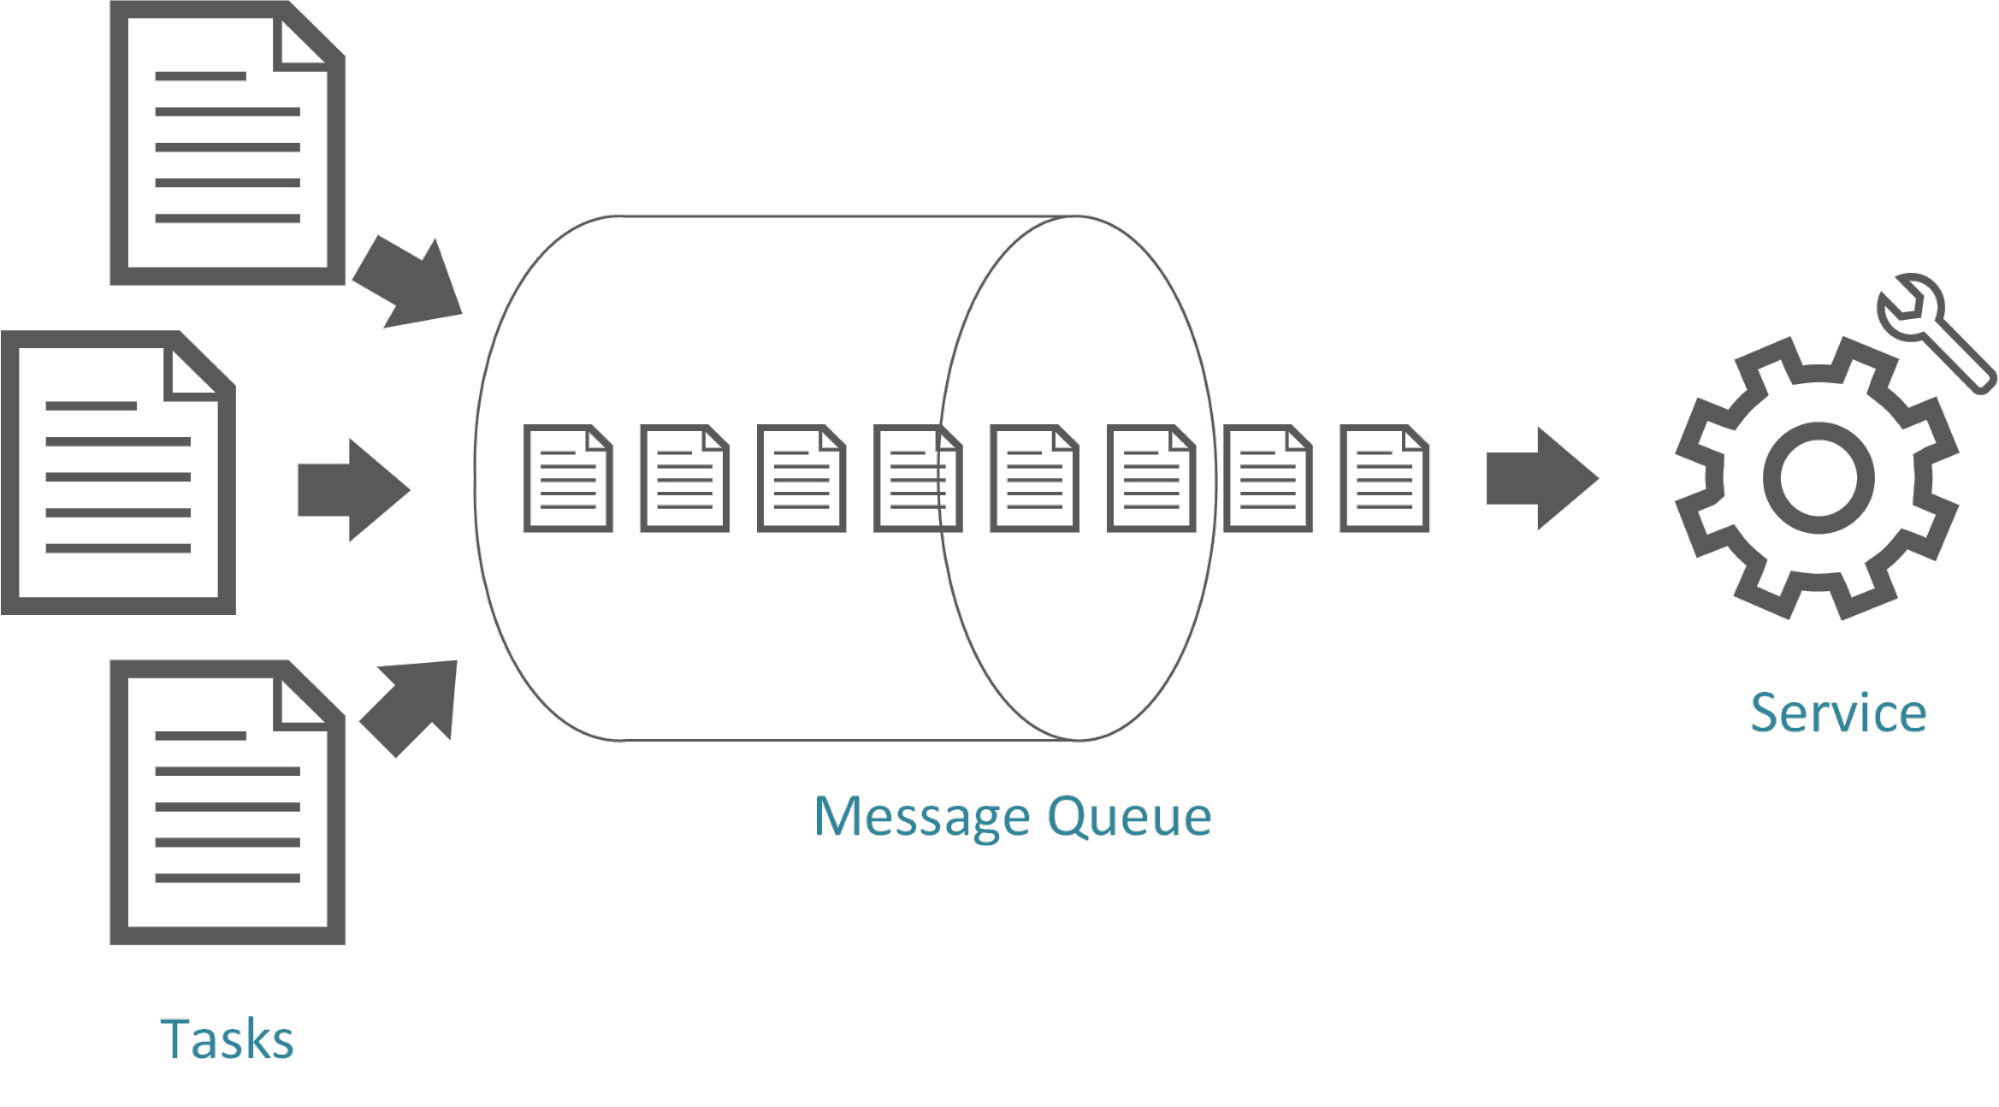
\includegraphics[width=\linewidth]{task_worker}
    \centering
    \caption{Tasks Worker}
    \label{fig:task_worker}
\end{figure}

\end{itemize}

\section{Variables}

Variables are the way to store data in The BPM and are used to exchange data between different tasks
and nodes.\\\\
Variables can be one of these data types
\begin{itemize}
    \item Booleans
    \item Strings
    \item Numbers
\end{itemize}
Many nodes have input and output fields that can be assigned to a variable that can change how this
node will behave.

\section{The BPM Cycle}

As stated before BPM works in a cycle and we will see how this cycle is executed in The BPM to execute business processes.
\\\\
The first thing the business will need to decide the business rules after deciding on the business rules the business will use our suit of applications.\\\\
Each Application works as stand alone application to execute part of the BPM cycle

\subsection{Designer}
\begin{figure}[h]
    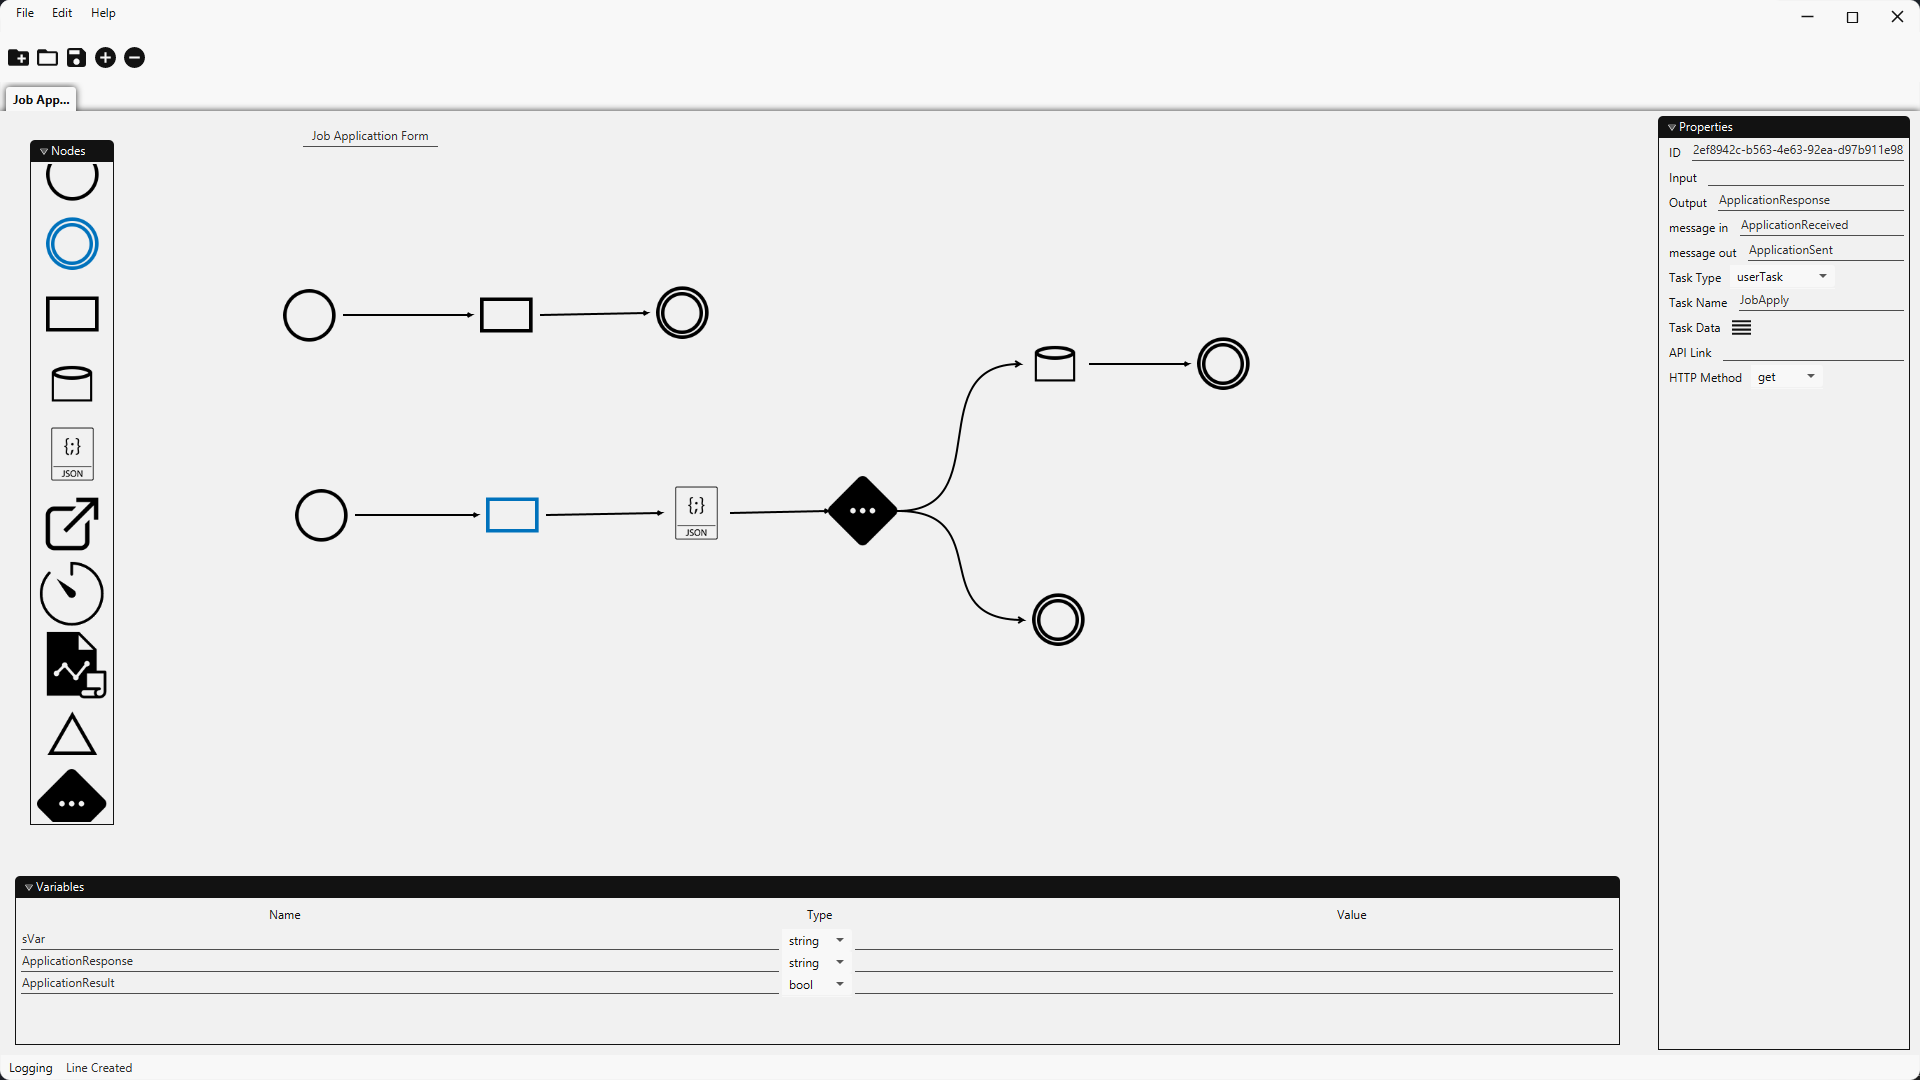
\includegraphics[width=\linewidth]{designer3}
    \centering
    \caption{Designer}
    \label{fig:designer}
\end{figure}

The designer is used to design the business process and adding variables to be initialized at run time
and modify how each node will behave.
It includes

\begin{itemize}
    \item A SQL editor to format SQL query for Database node, request editor for service task node
    \item A JSON Editor to define request or objects in JSON format and can also be used to read
    \item A User task editor to define tasks that need to be done by human actors
\end{itemize}

The designer enables the user to design the workflow, add variables to be added to run time and
properties window to change the nodes setting.\\\\
The process is then generated in an XML file format and the file is now ready for the engine to load
and execute.\\\\
Tools used to build designer
\begin{itemize}
    \item Java
    \item JavaFX 11 used to build the GUI as it allows you to create Java applications with a
    modern, hardware-accelerated user interface that is highly portable
    \item Gradle as a build system
\end{itemize}

\subsection{Engine}

The main system in the engine is the workflow engine which is used to execute the process by moving
the flow of execution from one node to another.\\\\
A workflow engine manages and monitors the state of activities in a workflow, such as the processing
and approval of a loan application form, and determines which new activity to transition to according
to defined processes (workflows). The actions may be anything from saving an application form in a
document management system to send a reminder email to users or escalating overdue items to
management. A workflow engine facilitates the flow of information, tasks, and events. Workflow
engines may also be referred to as Workflow Orchestration Engines.\\\\
Workflow engines mainly have these functions

\begin{itemize}
    \item Verification of the current process status: Check whether it is valid to execute a task, given
    current status
    \item Determine the authority of users - Check if the current user is permitted to execute the task
    \item Executing condition script: After passing the previous two steps, the workflow engine
    executes the task, and if the execution is completed successfully, it returns the success, if not,
    it reports the error to trigger and roll back the change
    \item A workflow engine is a core technique for task allocation software, such as business process
    management, in which the workflow engine allocates tasks to different executors while
    communicating data among participants. A workflow engine can execute any arbitrary
    sequence of steps, for example, a healthcare data analysis
\end{itemize}

The Engine has an API that enables other applications to use its functions and integrate them into their
systems and it is what the ERP uses to integrate The BPM inside it.\\\\

The API gives other applications the ability to manipulate workflow
\begin{itemize}
    \item Load, Start, alter and stop execution
    \item Get the tasks
\end{itemize}

Tools used to build engine
\begin{itemize}
    \item Java
    \item Gradle as a build system
\end{itemize}


\subsection{Monitor}

The Monitor is used to follow the execution of a process and can modify its execution, it helps give
users the ability to view the process and monitor it if anything went wrong or if there is a
bottlenecking anywhere in the process that needs to be modified and get an idea of how the process is
going\\\\
Tools used to build monitor
\begin{adjustwidth}{2cm}{}
    .Net core to be integrated easily with The ERP application\\
\end{adjustwidth}

\chapter{BPM Examples}

\section{Examples of Process-Based Applications}
The following examples are familiar to many organizations.\\\\
We will start with a simple example that shows how to model a simple business process.

\subsection{Bakery}
We want to model the following situation using BPMN 2.0. For a bakery which will start at the
beginning of each day. They will start by baking the bread then selling it and at the end of the day, all
the workers will receive their payments.

\begin{figure}[h]
    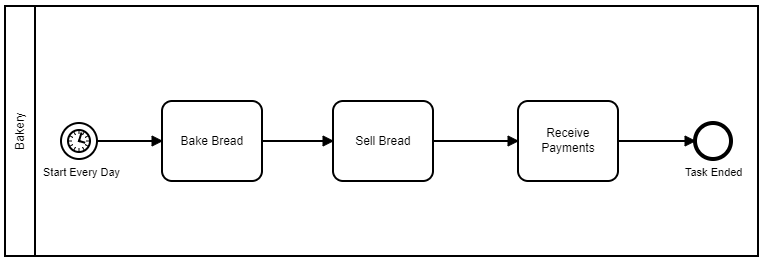
\includegraphics[width=100mm]{bakery}
    \centering
    \caption{Bakery Worflow}
    \label{fig:bakery}
\end{figure}

For our Implementation
\begin{figure}[h]
    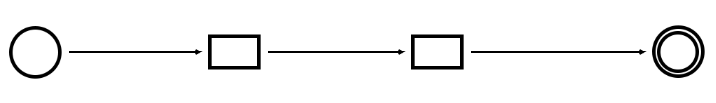
\includegraphics[width=100mm]{bpm_bakery}
    \centering
    \caption{Bakery Worflow}
    \label{fig:bpm_bakery}
\end{figure}



\subsection{Payment Request}
We will use the following example to illustrate how to model a two-step escalation using BPMN 2.0.
When we want a pizza, we order one. Sometimes the pizza delivery screws up and the delivery takes
longer than 20 minutes. Then we complain to the delivery service. After that, we give them another 30
minutes to deliver the pizza. If they do not make it in time, we give up and cancel our order.

\begin{figure}[h]
    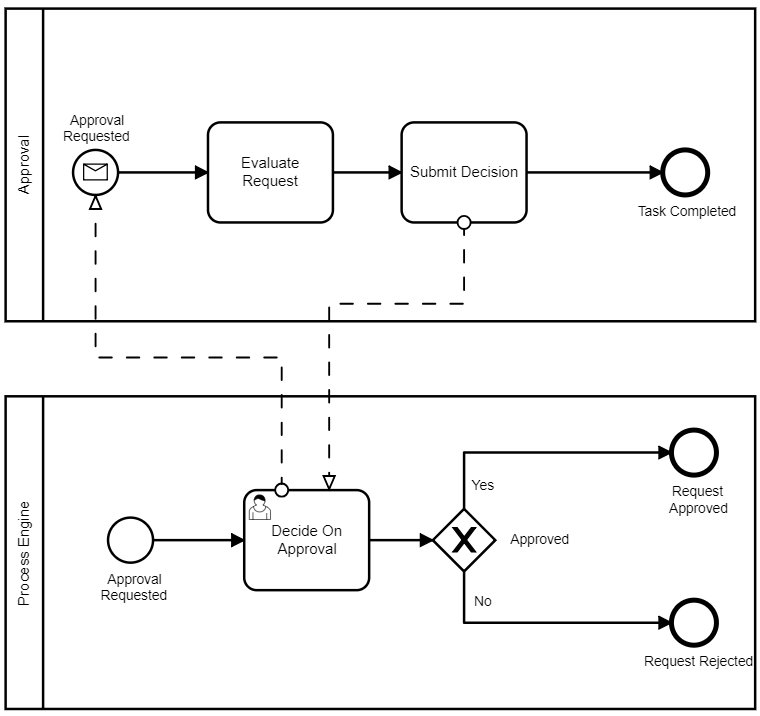
\includegraphics[width=80mm]{payment}
    \centering
    \caption{Payment Request Worflow}
    \label{fig:payment}
\end{figure}

For our Implementation
\begin{figure}[h]
    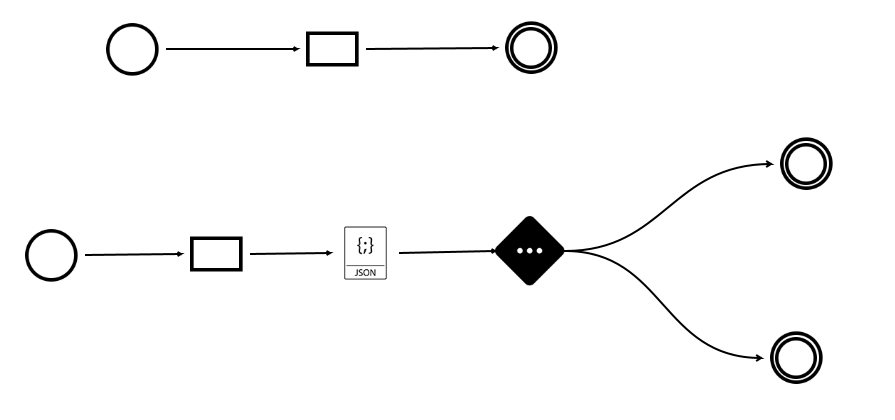
\includegraphics[width=100mm]{bpm_payment}
    \centering
    \caption{Bakery Worflow}
    \label{fig:bpm_payment}
\end{figure}